% Author: Dominik Harmim <harmim6@gmail.com>

\documentclass[a4paper, 11pt]{article}

\usepackage[czech]{babel}
\usepackage[utf8]{inputenc}
\usepackage[T1]{fontenc}
\usepackage{graphicx}
\usepackage[unicode, colorlinks, hypertexnames=false, citecolor=red]{hyperref}
\usepackage[left=2cm, top=3cm, text={17cm, 24cm}]{geometry}
\usepackage{wrapfig}


\interfootnotelinepenalty=10000

\graphicspath{{img/}}

\hypersetup{
    pdftitle={Dějiny a~filozofie techniky - Alan Turing},
    pdfauthor={Dominik Harmim <xharmi00@stud.fit.vutbr.cz>}
}

\title{\vspace{-4em}Alan Turing\vspace{-.5em}}
\author{%
    \textbf{Dominik Harmim} \texttt{<xharmi00@stud.fit.vutbr.cz>} \\
    Dějiny a~filozofie techniky\,---\,FIT VUT v~Brně%
}
\date{\vspace{-.5em}\today\vspace{-1em}}


\begin{document}


\maketitle


Při výběru tématu pro semestrální práci do kursu \emph{Dějiny a~filozofie
techniky} jsem se rozhodl pro popis života a~díla \emph{Alana Turinga},
jenž byl velmi významný \emph{matematik}, \emph{logik},
\emph{kryptoanalytik} a~zakladatel \emph{moderní informatiky}, který je mimo
jiné známy pro své zásluhy o~dešifrování nacistických tajných kódů během 2.
světové války. Je tedy podle mého názoru opravdu velice významná osoba na
poli dějin techniky a~jedena z~nejvýznamnějších osobností co se dějin moderní
informatiky týče.

Při psaní této práce jsem čerpal informace především z~přednášky Radka Tesaře
o~Alanu Turingovi z~roku 2014 konané na FIT VUT v~Brně\footnote{Záznam
přednášky Radka Tesaře o~\emph{Alanu Turingovi}:
\url{https://video1.fit.vutbr.cz/index.php?record_id=29166}.} a~z~článku
\emph{Alan Mathison Turing\,---\,život a~dílo}\footnote{\textsc{Tesař,~R.},
\textsc{Křivka,~Z.} a~\textsc{Meduna~A.} Alan Mathison Turing\,---\,život
a~dílo. \textit{Pokroky matematiky, fyziky a~astronomie}, roč.~59 (2014),
č.~2. S.~89--104. ISSN 0032-2423. Dostupné na:
\url{https://dml.cz/handle/10338.dmlcz/143889}.}.


\section{Mládí}

\begin{wrapfigure}{r}{.3 \linewidth}
    \centering
    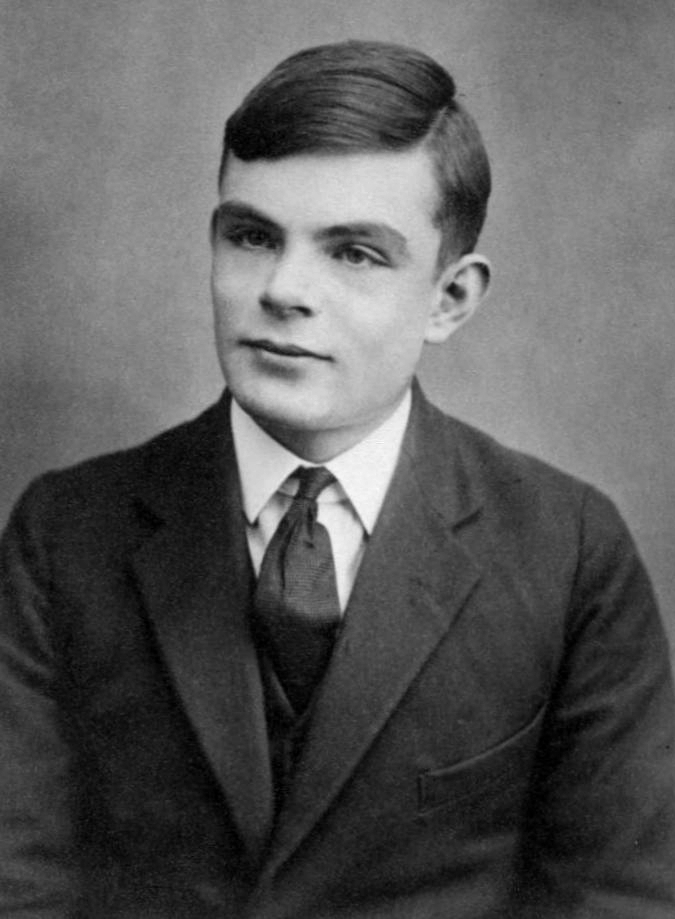
\includegraphics[width=.7 \linewidth]{turing.jpg}
    \caption{%
        Alan Turing cca v~roce 1927 \\
        \tiny{(\url{https://wikipedia.org/wiki/Alan_Turing})}%
    }
    \label{fig:turing}
\end{wrapfigure}

\emph{Alan Mathison Turing} (viz
obrázek~\ref{fig:turing}), který se narodil 23. června 1912 a~zemřel 7.
června 1954, byl významný britský \emph{matematik}, \emph{logik},
\emph{kryptoanalytik} a~zakladatel \emph{moderní informatiky}. Narodil se
v~Paddingtonu (Londýn). Rodiče Julius Mathison a~Ethel Sara Turingovi žili
téměř do Alanova narození (a~pak i~později) v~indickém Madrásu. Julius
a~Ethel však chtěli, aby Alan byl vychován v~Anglii. Otec Julius byl syn
kněze  ze skotské rodiny obchodníků, která pocházela z~Holandska. Matka
Ethel byla dcera hlavního inženýra Madráských železnic. Její rodina byla
protestantská anglo-irská šlechtická rodina pocházející z~hrabství Tipperary
a~Longford. Z~její rodiny pocházelo v~19. století hned několik významných
fyziků a~inženýrů. Poté, co se Alan narodil, se jeho otec vrátil z~Anglie
zpět do Indie a~matka jej následovala o~rok a~půl později, ale malého
Alana s~sebou nevzali, vychovávali ho chůvy a~příbuzní. Když Alanův otec
odešel do výslužby, oba rodiče opustili Indii a~usadili se na francouzské
straně kanálu La Manche.

Alan ve svém dětství nevykazoval výjimečnou inteligenci. Bavily ho šachy,
ale nebyl zvlášť dobrým hráčem. Ve věku 14 let se dostal na střední školu
v~Sherborne, která ho ale zklamala. Byl neohrabaný ve vztazích se spolužáky
a~učiteli, proto se často stával terčem posměchu. Jediné, co ho zajímalo,
byly \emph{přírodní vědy}. Nadchla ho také chemie, ale hlavně
\emph{matematika}. I~přes kritiku učitelů Turing často vytvářel vlastní
postupy řešení problémů. Pro své nekonvenční myšlení Turing vyhrával téměř
všechny matematické soutěže v~Sherborne. V~chemii, která ho zaujala od
velmi útlého věku, prováděl své vlastní pokusy, kterým se pak věnoval v~průběhu
celého svého života a~ve své chemické laboratoři trávil hodně času. Během
své školní docházky se také věnoval pokročilé matematice\,---\,četl práce
\emph{Alberta Einsteina} o~\emph{teorii relativity} a~práci \emph{Arthura S.
Eddingtona} o~\emph{kvantové mechanice}.

Na škole se seznámil s~\emph{Christopherem Morcomem}, ~s~nímž ho pojilo
hluboké přátelství, které později přecházelo v~mnohem hlubší city. Zde si
pravděpodobně poprvé uvědomil své \emph{homosexuální zaměření}. Když v~roce
1930 Morcom zemřel na tuberkulózu, byla to pro Turinga rána. Poté
se Turing rozhodl plně věnovat vědě. Protože Morcom byl před svou smrtí
přijat na \emph{Cambridge}, rozhodl se Alan naplnit jeho odkaz. Podle svých
slov chtěl učinit objevy, které by jinak jistě učinil Morcom.

Rok po Moromově smrti byl přijat na \emph{King's College} v~Cambridgi, kde
působili Bernard Russell, Alfred N. Whitehead a~Ludwig Wittgenstein.
Odehrávaly se zde debaty o~zásadních otázkách \emph{matematiky}
a~\emph{logiky}. Od roku 1933 ho zde začala zajímat matematická logika,
a~proto zde v~prosinci téhož roku přečetl svoji práci \emph{Matematika
a~logika}, v~níž tvrdil, že na matematiku se nelze dívat jen čistě logicky,
ale že matematika vyžaduje různé interpretace, jichž nelze logikou dosáhnout.

V~letech 1931--1934 studoval hlavně matematiku a~v~roce 1935 byl zvolen
členem univerzitní koleje na základě své disertace \emph{O~Gaussově
chybové funkci}, v~níž dokázal některé zásadní věty o~\emph{teorii
pravděpodobnosti} jako je \emph{centrální limitní věta}. Přestože tato
byla objevena krátce před Turingovou prací, Turing tuto větu
objevil a~dokázal nezávisle. V~roce 1936 pak obdržel \emph{Smithovu cenu}.
Turingovo zaměření a~vědecký přínos se tak netýká pouze \emph{informatiky},
i~když je v~této oblasti nejvýznamnější.

Roku 1935, když začal navštěvovat přednášky \emph{Maxe Newmana} o~základech
matematiky, se začal zabývat prací \emph{Kurta Gödela} o~\emph{neúplnosti}
a~\emph{Hilbertovým problémem rozhodnutelnosti}. Jeho největší zásluhy
tkví v~jeho článku z~roku 1936, ve kterém zavedl pojem \emph{Turingova
stroje}\,---\,teoretického modelu obecného výpočetního stroje\,---\,který
se stal jedním ze základů informatiky, a~dokázal, že \emph{problém zastavení}
Turingova stroje \emph{není rozhodnutelný}. Na základě
\emph{Churchovy-Turingovy teze} pak lze toto zjištění aplikovat na
Hilbertem formulovaný problém rozhodnutelnosti. Gödel zveřejnil v~roce 1931
věty o~neúplnosti, které matematiky tehdejší doby doslova šokovaly. Tyto
věty zjednodušeně říkají, že v~matematice \emph{není dokazatelné vše}.
Turing svým strojem dokázal, že Gödelova tvrzení jsou pravdivá. Turing také
publikoval článek, který obsahuje teoretické základy ke konstrukci
\emph{počítače} a~k~\emph{programování}.

V~roce 1936 se Turing stal postgraduálním studentem na Princetonské
univerzitě, kde byl členem výzkumného týmu matematický logiků vedených
\emph{Alonzem Churchem}. Pracoval mimo jiné na \emph{komplexní analýze}
a~\emph{Riemannově funkci zeta}\footnote{Jedná se o~platnost \emph{Riemannovy
hypotézy}, která se týká \emph{netriviálních nulových bodů} funkce zeta.
Turing se snažil ověřit platnost hypotézy. V~této oblasti učinil významný
pokrok. Do dnešního dne nebyla Riemannova hypotéza ani potvrzena ani
vyvrácena. Všechny výpočty netriviálních bodů až do dnešní doby se provádí
\emph{Turingovou metodou}. Na tento problém vypsal Clayův matematický institut
odměnu 1\,000\,000 amerických dolarů za jeho potvrzení nebo vyvrácení.}.
V~roce 1938 dokončil svoji práci o~logice a~obhájil doktorát.


\section{Enigma}

Nejdůležitější část Turingova života se odehrávala za války, kdy
v~\emph{Bletchley Parku} prováděl \emph{kryptoanalýzu}. Zde se také dočkal
největšího uznání svých kolegů a~byla to práce, která jej zcela pohltila.

\emph{Enigma} je \emph{šifrovací přístroj}, který vytvořil německý vynálezce
\emph{Arthur Scherbius} roku 1918. Tisíce kusů tohoto přístroje se prodaly
německé armádě, která ho používala pro šifrování své komunikace. Enigmu lze
nastavit pomocí \emph{propojovací desky} a~\emph{rotorů}. Nastaveným
přístrojem je možné zašifrovat určitou zprávu, v~zašifrované podobě ji
odeslat a~následně opět dešifrovat stejně nastavenou Enigmou. Počet možností,
jak Enigmu nastavit, je více než $ 10^{16} $. Scherbius tudíž nabyl
přesvědčení, že Enigma je nezdolatelná. Němci navíc nastavení jednotlivých
strojů každý den měnili.

Luštit Enigmu začal v~Polsku matematik \emph{Marian Rejewski} ještě před
druhou světovou válkou. Sestavil několik mechanických strojů (tzv.
\emph{bomby}), které dokázaly zjistit správné nastavení Enigmy. V~roce 1938
Němci zvýšili bezpečnost Enigmy, čímž ztížili dešifrování, a~proto Poláci
předali dosavadní výsledky Britům, kteří v~kryptoanalýze pokračovali. Práce
pokračovala v~Anglii v~Bletchley Parku, kam v~roce 1939 nastoupil Turing
a~hned se vrhl na rozvíjení práce Rejewského. Turing začal stavět stroj
podobný bombě, kterou postavil Rejewski. Turing byl v~Bletchley Parku považován
za prvotřídního odborníka a~génia, ale nikdo mimo neměl ani ponětí o~jeho
pozoruhodném výkonu, protože vše, co s~touto prací souviselo, bylo přísně
tajné. Němci opět jistým způsobem zvýšili bezpečnost Enigmy. Roku 1940 však
Turing postavil novou bombu, která byla schopna nastavení stroje zjistit.
Angličané měli po větší část války k~dispozici většinu z~tajné nepřátelské
komunikace. Podle sira Harryho Hinsleye zkrátila Turingova práce válku
nejméně o~tři roky a~byly díky ní zachráněny tisíce životů.

Němci nespoléhali jen na Enigmu. Měli také sofistikovanější šifru
\emph{Lorenz}, kterou šifrovali pomocí stroje \emph{Tunny}. Pro kryptoanalýzu
Turing roku 1943 sestrojil \emph{Colossus}\,---\,první \emph{elektronický
počítač} na světě. Jednalo se o~první \emph{programovatelný počítač} na světě.
Protože vše, co se tohoto týkalo, bylo přísně tajné, byl Colossus po válce
zničen a~nesmělo se o~něm mluvit. Proto bylo prvenství elektronického
počítače přiřknuto univerzitě v~Pensylvánii, kde v~letech 1943--1946
vytvořili \emph{ENIAC}.

V~letech 1941--1942 byl Turing vyslán do USA, aby se zde podílel na dekódování
německých zpráv. Němci později změnili své kódy a~kryptoanalytici v~Bletchley
Parku nemohli dále jejich zprávy dekódovat. Turing už se přímo nepodílel na
rozluštění těchto složitějších kódů, ale jeho myšlenky byly významným
přínosem. V~roce 1945 byl Turing za tento přínos vyznamenán. Po válce převzalo
veškeré dešifrovací aktivity z~Bletchley Parku centrum v~Londýně, které
zaměstnávalo Turinga až do roku 1952.


\section{Po válce}

V~roce 1947 se Turing vrátil do Cambridge, kde studoval \emph{neurologii}
a~\emph{fyziologii}. Od roku 1948 Turing přednášel na Univerzitě
v~Manchesteru. Pokládal si zásadní otázky týkající se dalšího rozvoje
počítačů. Také dlouhodobě uvažoval o~možnostech \emph{inteligentních strojů}
a~je autorem tzv. \emph{Turingova testu}, který tvrdí, že za inteligentní
můžeme stroj považovat tehdy, když nejsme schopni odlišit jeho výstup od
výstupu člověka. V~roce 1990 Hugh Loebner založil nadaci, jež prvnímu stroji,
který úspěšně složí Turingův test, udělí cenu a~100\,000 amerických dolarů.
Do dnešního dne nebyla tato cena udělena.

Po druhé světové válce byly myšlenky Turingova stroje využity při konstrukci
prvních počítačů řízených programem uloženým ve \emph{vnitřní paměti}. Turing
byl považován za jednu z~největších autorit v~tomto oboru a~jeho teoretické
poznatky se v~USA začaly zhodnocovat i~v~praxi. Turing se také podílel
na vývoji počítačů \emph{Manchester Mark~I a~II}. Tyto počítače Turing
prakticky využíval v~50. letech, kdy pracoval na teoretickém vysvětlení
\emph{morfogeneze}. Na přelomu 40. a~50. let se zaměřil na studium
struktury mozku živých bytostí, což bylo poslední téma jeho životní kariéry.
V~roce 1951 pracoval na aplikaci matematické teorie na biologické formy,
kterou se zabýval až do konce svého života. Zabýval se také myšlenkami
\emph{kvantové teorie}, reprezentací \emph{elementárních částic}
a~\emph{teorií relativity}. Za svoji práci o~Turingově stroje v~roce 1936 se
Turing v~roce 1951 stal členem Královské společnosti v~Londýně.

V~roce 1952 se policie dozvěděla o~Turingově \emph{homosexualitě}, což bylo ve
Velké Británii až do roku 1994 trestné. Kvůli tomu mu byla zrušena
bezpečnostní prověrka a~skončila tedy i~jeho práce pro Vládní komunikační
centrum. Turing představoval pro britskou bezpečnostní službu vážné
nebezpečí, protože měl řadu zahraničních kolegů po celém světě. Policie
začala tajně sledovat jeho zahraniční návštěvy. Turing byl zatčen a~v~březnu
roku 1952 odsouzen a~musel volit mezi ročním vězením
a~probací\,---\,podmíněným prominutím trestu, které ovšem bylo vázáno na
podstoupení roční hormonální \uv{léčby}. Rozhodl se pro druhou možnost
a~po dobu jednoho roku dostával ke snížení libida dávky estrogenu.

Dne 7. června 1954 Turing zemřel na \emph{otravu kyanidem}. Tím mělo
být napuštěno jablko, kterého několik soust snědl. Přítomnost kyanidu v~jablku
však nebyla testována. Jako příčina smrti byl kyanid určen až při pitvě.
Podle oficiálního stanoviska se jednalo o~sebevraždu, čímž byly odmítnuty
spekulace o~náhodě, nebo o~vraždě. Někteří autoři ale mluví o~Turingově
smrti spíše jako o~\emph{vraždě na vládní příkaz}.


\section{Současnost}

Na počest Alana Turinga je od roku 1966 udílena \emph{Turingova
cena}\,---\,jedno z~nejvýznamnějších informatických ocenění. V~roce 1999
časopis \emph{Time} označil Turinga jako jednoho ze 100 nejdůležitějších
lidí 20. století za jeho přínos k~rozvoji \emph{umělé inteligence}
a~\emph{moderních počítačů}.

V~září 2009 se britský premiér Gordon Brown jménem vlády omluvil Alanu
Turingovi za příkoří, které mu bylo způsobeno, když byl odsouzen pro
homosexualitu. Dne 24. prosince 2013 byla Alanu Turingovi udělena
\emph{královská milost}. Byl tím zbaven všech obvinění. \uv{\emph{Doktor Alan
Turing byl mimořádný muž s~mimořádnou myslí. Jeho genialita pomohla ukončit
válku a~zachránila tisíce životů. Jeho pozdější život byl zastíněn jeho
odsouzením za homosexualitu. Tento rozsudek bychom nyní považovali za
nespravedlivý a~diskriminační, a~proto byl rozsudek odvolán. Turing si
zaslouží být uznáván za své přínosy ve válečném tažení a~ve vědě o~počítačích.
Milost od královny je adekvátní hold tomuto skvělému muži.}}, řekl k~milosti
tehdejší ministr spravedlnosti Velké Británie Chris Grayling.


\end{document}
